\documentclass[11pt]{amsart}
\usepackage{amsaddr}
\usepackage{mathtools}
\usepackage{aas_macros} % macro pour Bibtex
\usepackage{hyperref}
\usepackage{graphicx} % Required for inserting images
\usepackage{amsthm}
\usepackage{amsmath}
% \usepackage{makecell}
\usepackage{amssymb}
\usepackage{enumitem}
\usepackage{color}
\usepackage{subcaption}



\usepackage{booktabs}
\usepackage{pifont}
\usepackage{natbib,fancyhdr} %new
\usepackage{bm}

%%%
\usepackage{tikz}
\usetikzlibrary{calc}
\usetikzlibrary{automata}
\usetikzlibrary{positioning}  %                 ...positioning nodes
\usetikzlibrary{arrows}   
\tikzset{stretch/.initial=1}    %                 ...customizing arrows
\newcommand\drawloop[4][]%
   {\draw[shorten <=0pt, shorten >=0pt,#1]
      ($(#2)!\pgfkeysvalueof{/tikz/stretch}!(#2.#3)$)
      let \p1=($(#2.center)!\pgfkeysvalueof{/tikz/stretch}!(#2.north)-(#2)$),
          \n1= {veclen(\x1,\y1)*sin(0.5*(#4-#3))/sin(0.5*(180-#4+#3))}
      in arc [start angle={#3-90}, end angle={#4+90}, radius=\n1]%
   }
\usepackage{tikz-cd}
\usetikzlibrary{cd}
%
%%%


%\usepackage{mathtools} % psmallmatrix

\newcommand{\cmark}{\ding{51}}%
\newcommand{\xmark}{\ding{55}}%

\setlength{\heavyrulewidth}{3\lightrulewidth}
\setlength{\abovetopsep}{1ex}

\newcommand{\Esp}[0]{\ensuremath{\mathbb{E}}}
\newcommand{\DKL}[0]{\ensuremath{\mathbb{D}_{\mathsf{KL}}}}

\DeclareMathOperator*{\argmax}{arg\,max}
\DeclareMathOperator*{\argmin}{arg\,min}
\DeclareMathOperator{\diag}{diag}

\usepackage[top=3cm, bottom=2cm, left=3cm, right=2cm]{geometry} %margins

% \usepackage{geometry}
%  \geometry{
%  a4paper,
%  left=25mm,
%  }

\newcommand{\jessa}[1]{{\color{red} #1}}
\newcommand{\field}[1]{\mathbf{#1}}
\newcommand{\nn}{\nonumber}


% My definitions:
\def\U{\mathcal U}
\def\LL{\mathcal L}
\def\P{\mathcal P}
\def\D{\mathcal D}

\DeclarePairedDelimiter\ceil{\lceil}{\rceil}
\DeclarePairedDelimiter\floor{\lfloor}{\rfloor}

% My packages:
\usepackage{algorithmic}
\usepackage[ruled,vlined,linesnumbered]{algorithm2e}
\usepackage{xcolor}
\usepackage{multicol} 
\usepackage{enumitem}
\newcommand\mycommfont[1]{\footnotesize\ttfamily\textcolor{blue}{#1}}
\SetCommentSty{mycommfont}
\newcommand{\bl}[1]{{\color{blue} #1}}
\newcommand{\rd}[1]{{\color{red} #1}}


% Alternative Assumption!

\newtheorem{theorem}{Theorem}
\newtheorem{assumption}[theorem]{Assumption}
\newtheorem{lemma}[theorem]{Lemma}
\newtheorem{corollary}[theorem]{Corollary}
\newtheorem{proposition}[theorem]{Proposition}
\newtheorem{fact}[theorem]{Fact}
\newtheorem{definition}{Definition}

% New environment
\newenvironment{assumptionp}[1]{
  \renewcommand\theassumptionalt{#1}
  \assumptionalt
}{\endassumptionalt}

\graphicspath{{./figures}}
\usepackage[margin=1cm]{caption}



\title{Galaxy image statistical generator: how to be confident?}
\author{Jean-Eric Campagne}
\address{Université Paris-Saclay, CNRS/IN2P3, IJCLab, 91405 Orsay, France
}
\email{jean-eric.campagne@ijclab.in2p3.fr}
\date{\today}
\calclayout  % switch off left right margin different even/odd pages.

\begin{document}
\maketitle
%\renewcommand{\baselinestretch}{0.75}\normalsize
%\tableofcontents
%\renewcommand{\baselinestretch}{1.0}\normalsize
%
\begin{abstract}
blabla
\\
\smallskip
\noindent \textbf{Keywords.} diffusion models, U-Net
\end{abstract}

\section{Introduction}
\label{sec:Intro}
Image generation in Machine Learning (ML) is a challenging task that has made a dramatic rise in quality recently thanks to the large scale statistical model architectures as for instance \texttt{DALL-E 2} \citep{ramesh2022}, \texttt{Midjourney} \citep{Oppenlaender2022} and \texttt{StableDiffusion} \citep{Rombach2022} which use \textit{stochastic diffusion processes}. Such models have replaced the previous generation based on \textit{variational auto encoder} (aka VAE) \citep{Kingma2014}\footnote{nb. notice that \texttt{arxiv} paper have been updated in 2022.} and  \textit{adversarial networks} (aka GAN) \citep{goodfellow2014generative} as in \citep[e.g.]{KarrasALL18,brock2018large}, or \textit{normalizing flows} (hereafter nicknamed NF) such as in \texttt{Glow} \citep{Kingma2018}. 


The ability of generative models have been rapidly adopted in many domains. For instance, in High Energy Physics the reader may be interested by the review \cite{PhysRevD.107.076017}. Concerning Astrophysics and Cosmology the generative models are used in different tasks (e.g. deblending \citep{Hemmati_2022,Arcelin2020} {\color{red} à compléter}) and especially to create synthetic galaxy images of complex morphologies going beyond parametrized analytic light profile simulations (eg. \texttt{GalSim} by \cite{ROWE2015121}). Along this line \citep{ravanbakhsh2016,Fussell2019} use GAN models, \cite{Lanusse2021} propose an hybrid VAE-Normalizing Flow architecture and \cite{smith2021} use a denoising stochastic diffusion model. 

Despite the impressive image quality of these generative models that are nowadays well diffused in the general public, many questions arise from mathematical and usage point of views. Notably, one may ask for what is really learned by the generative models and what are the statistical properties of the generated samples. In a general manner \cite{Hataya2023} ask if the image generated can corrupt the future datasets. However, the study is devoted  to the large scale statistical models mentioned above that are trained usually with billion-scale data extracted from the Internet, and so in turn can be contaminated by the images shared by many users. Concerning galaxy image generation the datasets are much more modest for the time being (i.e $O(10^5)$) collected from optical surveys (eg. COSMOS HST Advanced Camera for Surveys, \cite{mandelbaum_2019_3242143},  Sloan Digital Sky Survey \citep[SDSS;][]{sdss} Data Release 7 \citep{sdssdr7}) and used by a rather small community compared to social network followers which certainly  limits the datasets corruption. So, besides image corruption, \cite{HACKSTEIN2023100685,janulewicz2024assessing} have investigated different metrics to address the question of fidelity of the generated galaxy images and morphological properties compared to the original dataset.

\cite{kadkhodaie2024generalization} address more mathematically oriented questions and demonstrate the passage between memorization to generalization of  diffusion generative models when the dataset size increases and propose interpretation of what is learned by the network as a sort of \textit{geometry-adaptive harmonic basis} going beyond the commonly used \textit{steerable wavelet basis} first introduced and studied in \cite{Simoncelli1995b,Unser2013} and developped for instance in the \texttt{Kyamato} library \citep{JMLR:v21:19-047}. The authors uses \textit{denoiser} architectures as \texttt{UNet} \citep{2015arXiv150504597R} and \texttt{BF-CNN} networks \citep{Mohan2020Robust} trained on \texttt{CelebA} \citep{Liu2015} and \texttt{LSUN} bedroom  \citep{Yu2015} reduced datasets of $O(10^5)$ images resized to $80\times 80$ pixels (grayscale). The dataset size and the number of pisels per image make possible to investigate how the \texttt{Glow} normalizing flow based model compare to denoiser based diffusion model concerning the generation of galaxy images both trained with the same dataset issued from DR7 SDSS survey.


In the following sections, first we briefly describe the different kind of generative models and we show the outcome of the conducted numerical experiment before drawing some guide lines. Appendix gives more details on the dataset used.
%
\section{Generative Models}
%
{\color{red} Mention ergodic vs non ergodic, reference Allys et al. Lempereur et al. simulation of ergodic case.}\hfill\\

The generative models assume that the observations $\bm{x}$ are described by a probability distribution $p(\bm{x})$ and aim to give a representation of such distribution.  It is also assumed that the data are i.i.d samples of $p(\bm{x})$.  In the following, it is not the intention to describe in high details the different  strategies and their implementations but rather {\color{red} to give some guide lines (à modifier)}.
%
\subsection{Variational Auto-Encoder}
%
Using \texttt{VAE} \citep{Kingma2014} means that it is assumed that there exists an underlying unobservable stochastic variable $\bm{z}$  (aka \textit{latent variable}) whose distribution is chosen \textit{a priori} among a parametrized distribution family $\pi_{\bm{\theta}_1}(\bm{z})$ differentiable both with respect to $\bm{z}$ and $\bm{\theta}_1$. In general the latent space has a much lower dimensionality than the data space which imply a information compression. Then, it yields $p(\bm{x}) = p(\bm{x}|\bm{z})\pi_{\bm{\theta}_1}(\bm{z})$. However, the likelihood  $p(\bm{x}|\bm{z})$ is also unknown which leads to the introduction of a parametrized version $p_{\bm{\theta_2}}(\bm{x}|\bm{z})$ with the differentiability properties as $\pi_{\bm{\theta}_1}$. Using the notation $\bm{\theta}=(\bm{\theta_1},\bm{\theta_2})$,  these parameters are adjusted in such a way that  $p_{\bm{\theta}}(x)$ matches the empirical distribution of the $N$ data samples ($\{\bm{x}^{i}\}_{i<N}$). The best solution $\bm{\theta}_{ML}$ is the maximum of $p_{\bm{\theta}}(x)$ but in practice this leads to  intractable problem (either analytical or numerical) as one should evaluate the gradient with respect to $\bm{\theta}$ of the integral 
$\int p_{\bm{\theta}_2}(\bm{x}|\bm{z})\pi_{\bm{\theta}_1}(\bm{z}) dz$ \citep{Kingma2014}. To overcome such problem, one uses first the Bayes relation
\begin{equation}
p_{\bm{\theta}}(x) p(\bm{z}|\bm{x}) = p_{\bm{\theta}_2}(\bm{x}|\bm{z})\pi_{\bm{\theta}_1}(\bm{z})
\end{equation}
and second a parametrized version of the unknown true \textit{a posteriori} distribution as $p_{\bm{\phi}}(\bm{z}|\bm{x})$. If one introduces the Kullback-Leibler divergence $\DKL(p\| q)=\Esp_{\bm{x}\sim p}[\log(p(\bm{x})/q(\bm{x}))]$, then taking the expected value according\footnote{We represent the sampling of variates $\bm{x}$ from a
distribution $p(\bm{x})$ using the notation $\bm{x}\sim p(\bm{x})$.} to $\bm{z}\sim p_{\bm{\phi}}(\bm{z}|\bm{x})$ of the both sides of the following expression
\begin{align}
\log p_{\bm{\theta}}(x) &= \log p_{\bm{\theta}_2}(\bm{x}|\bm{z}) + \log \pi_{\bm{\theta}_1}(\bm{z}) - \log p(\bm{z}|\bm{x}) + \log p_{\bm{\phi}}(\bm{z}|\bm{x}) - \log p_{\bm{\phi}}(\bm{z}|\bm{x})
\end{align}
yields 
\begin{align}
\log p_{\bm{\theta}}(x)  &= \Esp_{z\sim p_{\bm{\phi}}}[\log p_{\bm{\theta}_2}(\bm{x}|\bm{z})] - \DKL(p_{\bm{\phi}}(\bm{z}|\bm{x})\| \pi_{\bm{\theta}_1}(\bm{z})) + \DKL(p_{\bm{\phi}}(\bm{z}|\bm{x})\| p(\bm{z}|\bm{x}))
\geq \mathcal{L}(\bm{x};\{\bm{\theta},\bm{\phi}\})
\label{eq-VAE-ELBO}
\end{align}
where we have emphasized the \textit{evidence lower bound} (aka ELBO)
\begin{equation}
\mathcal{L}(\bm{x};\{\bm{\theta},\bm{\phi}\}) = \Esp_{z\sim p_{\bm{\phi}}}[\log p_{\bm{\theta}_2}(\bm{x}|\bm{z})] - \DKL(p_{\bm{\phi}}(\bm{z}|\bm{x})\| \pi_{\bm{\theta}_1}(\bm{z}))
\end{equation}
and use the positiveness property of the $\DKL$ divergence. Maximizing with respect to 
$\{\bm{\theta},\bm{\phi}\}$ the ELBO is now tractable as it is free of the unknown distributions $p(\bm{x})$ and $p(\bm{z}|\bm{x})$. However, the gradient with respect to $\phi$ may experience large variance, so \cite{Kingma2014} have introduced an auxiliary  variable $\varepsilon$ such that $\bm{z}\sim p_{\bm{\phi}}(\bm{z}|\bm{x})$ is replaced by $\bm{z} = g_{\bm{\phi}}(\bm{\varepsilon},\bm{x})$ with $\bm{\varepsilon} \sim p(\bm{\varepsilon})$ and $g_{\bm{\phi}}(\bm{\varepsilon},\bm{x})$ a differentiable function with respected to $\phi$. 

It is usual to call $p_{\bm{\theta}_2}(\bm{x}|\bm{z})$ the \textit{decoder} part of the whole model while $p_{\bm{\phi}}(\bm{z}|\bm{x})$ is the \textit{encoder} part. The different VAE models differ by the distribution families used. The simplest choice may be commonly-used Gaussian multivariate distributions, and the centred isotropic with unit variance version ($\mathcal{N}(\bm{z},\bm{0},\bm{1}$) for the $\bm{z}$ prior (nb. $\bm{\theta}_1$ are missing is this scenario). Once the optimization is done, the \textit{decoder} is used as a $\bm{x}$ generator by feeding with $\bm{z}$ samples. It turns out that simple VAE tends to generate blurry images and may  suffer from the problem of \textit{posterior collapse} which motivate active ML researches \citep[e.g.][]{engel2018latent,Takida2022} and modified VAE versions to overcome this issue as for instance in \cite{Lanusse2021}. 
%
\subsection{Generative Adversarial Networks}
%
The vanilla GAN \citep{goodfellow2014generative} shares with VAE the target to optimize a \textit{generator} network ($\bm{G}$) to get $\bm{x}$ samples from a latent variable $\bm{z}$ such that  $\bm{x} = \bm{G}(\bm{z})$ with $\bm{z}$ \textit{prior} $\pi(\bm{z})$ is for instance a Gaussian distribution $\mathcal{N}(\bm{z},\bm{0},\bm{1})$. To do so, a second network ($\bm{D}$) acts as a \textit{discriminator} which aims to state if a sample $\bm{x}$ is from the model distribution or the data distribution. To reach that goal one solves the \texttt{min-max} problem
\begin{equation}
\min_{\bm{G}} \max_{\bm{D}}\left\{ \Esp_{\bm{x}\sim p_{data}(\bm{x})}[\log \bm{D}(\bm{x})] + \Esp_{\bm{z}\sim \pi(\bm{z})}[\log(1-\bm{D}(\bm{G}(\bm{z})))] \right\}
\end{equation} 
where $p_{data}$ is the data generating distribution. Both the  $\bm{G}$ and $\bm{D}$ are parametrized networks. Notice that at parameter of $\bm{G}$ fixed, the optimal \textit{discriminator} $\bm{D}^\ast$ has the following expression
\begin{equation}
\bm{D}^\ast(\bm{x}) = \frac{p_{data}(\bm{x})}{p_{data}(\bm{x}) + p_{\bm{G}}(\bm{x})}
\end{equation}
with $p_{\bm{G}}(\bm{x}) = \pi(\bm{z})|\det J_{\bm{G}} |^{-1}$ using the Jacobian of the \textit{generator}, leading to a reformulation of the \texttt{min-max} problem as followed
\begin{equation}
\min_G \left\{ \DKL{\left( p_{data} \left\| \frac{p_{data} + p_{\bm{G}}}{2}\right. \right) }  + \DKL{\left(p_{\bm{G}} \left\| \frac{p_{data} + p_{\bm{G}}}{2} \right. \right)} \right\}
\end{equation}
leading to the optimal solution $p_{\bm{G}} = p_{data}$ yielding a perfect matching of the data distribution. 
%
\subsection{Normalizing Flows}
%
Looking at Equation \ref{eq-VAE-ELBO}, one notices that the optimal solution is reached in case of $\DKL(p_{\bm{\phi}}(\bm{z}|\bm{x})\| p(\bm{z}|\bm{x}))=0$ which is true iif $p_{\bm{\phi}}(\bm{z}|\bm{x}) = p(\bm{z}|\bm{x})$. But this situation cannot be true in general as typical $p_{\bm{\phi}}$ parametrizations involve for instance independent Gaussian distributions. The limited choices of the parametrization is one of the limitation of VAE. So, one motivates the use of normalizing flows (NF) to allow for more flexibility in the distribution family design to hope that the true posterior is member of such family \citep{Tabak2010, Tabak2013a, Rezende2015}. 

Independently of the VAE context, a flow $T$ is defined as diffeomorphism (aka bijector) between the data space and a latent space such that
\begin{align}
\bm{x} = T(\bm{z}) & \quad \Leftrightarrow \quad \bm{z} = T^{-1}(\bm{x})
\end{align}
So, if $\bm{z}$ distribution is $\pi(\bm{z})$ (e.g. $\mathcal{N}(\bm{z},\bm{0},\bm{1})$) then the following relation apply
\begin{equation}
p(\bm{x}) =  \pi(\bm{z})|\det J_T(\bm{z})|^{-1} = \pi(T^{-1}(\bm{x}))|\det J_{T^{-1}}(\bm{x})|
\end{equation}
Contrary to VAE and GAN the latent and data space dimensionalities are the same. The flow $T$ is in general a composition of several individual flows $\{T_i\}_{i<n}$ in such a way that
\begin{align}
T=T_1\circ T_2\circ \dots \circ T_n & \quad \Leftrightarrow \quad 
T^{-1}=T_n^{-1}\circ T_{n-1}^{-1}\circ \dots \circ T_1^{-1}
\end{align}
Figure \ref{fig-normflow} represents a schematic views of the \textit{forward} or \textit{generative} direction and the \textit{backward} or \textit{training} direction. 
If one notes $\bm{z}_i = T_i(\bm{z}_{i-1})$ for all $i<n$  (using $\bm{z}_0=\bm{z}$, $\bm{z}_n=\bm{x}$) then
\begin{equation}
\log |\mathrm{det} J_T| = \sum_{i=0}^{n-1} \log |\det J_{T_i}(\bm{z}_{i-1})|
\label{eq-flow-jacob}
\end{equation}
Theorem exists showing that under moderate assumptions flow-based models are able to represent any density distributions \citep{Bogachev2005,huang2019solving}. So, if the flows are well chosen, one can sample $\bm{x}$ with potentially complex (multi-modes) density distribution from a simple spherical centred multivariate Gaussian distribution.


%
\begin{figure}
\resizebox{0.8\columnwidth}{!}{%
%\begin{center}
\begin{tikzpicture}[
node distance = 1cm, 
distrib/.style={rectangle},
]

\node[state] (s0) {$z$};
\node[distrib, above=0.1cm of s0] (img0) {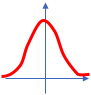
\includegraphics[height=1cm]{fig-nf-z.png}}; 
\node[state, right = of s0] (s1) {$z_1$};
\node[state, right = of s1] (sim1) {$z_{i-1}$};
\node[state, right = of sim1] (si) {$z_{i}$};
\node[distrib, above=0.1cm of si] (imgi) {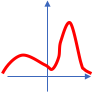
\includegraphics[height=1cm]{fig-nf-zi.png}}; 
\node[state, right = of si] (snm1) {$z_{n-1}$};
\node[state, right = of snm1] (sn) {$x$};
\node[distrib, above=0.1cm of sn] (imgx) {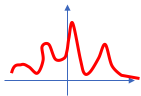
\includegraphics[height=1cm]{fig-nf-x.png}}; 

\path[-Stealth]
	(s0) edge[bend left] node [above] {$T_1$} (s1)
	(s1) edge[bend left] node [below] {$T_1^{-1}$} (s0)
	(s1) edge[dotted, ultra thick,-] (sim1)
	(sim1) edge[bend left] node [above] {$T_i$}  (si) 
	(si) edge[bend left] node [below] {$T_i^{-1}$}  (sim1) 
	(si) edge[dotted, ultra thick,-](snm1)
	(snm1) edge[bend left] node [above] {$T_n$}  (sn)
	(sn) edge[bend left] node [below] {$T_n^{-1}$}  (snm1); 

\end{tikzpicture}}
\caption{Schematic Normalizing Flow scheme inspired by \cite{weng2018flow}. On the top the \textit{forward} or \textit{generative} direction from a simple $\bm{z}$ distribution to a more complex one for $\bm{x}$. On the bottom the \textit{backward}  or \textit{training} direction from complex to simple distributions.}
\label{fig-normflow}
\end{figure}
%

Let the flow be parametrized by a vector $\bm{\theta}$ leading to a parametrized flow-model $p_{\bm{\theta}}(\bm{x})$. To obtain an optimized flow, we consider the $\DKL$ divergence between  $p_{\bm{\theta}}(\bm{x})$ and the true $p(\bm{x})$ leads to (n.b we consider $\pi(\bm{z})=\mathcal{N}(\bm{z}, \bm{0}, \bm{1})$ without any extra unknown parameters)
\begin{align}
\mathcal{L}(\bm{\theta}) &= \DKL(p(\bm{x})\|p_{\bm{\theta}}(\bm{x}))
= - \Esp_{\bm{x}\sim p(\bm{x})}[-\log p_{\bm{\theta}}(\bm{x})] + \mathrm{const.} \nn \\
&= - \Esp_{\bm{x}\sim p(\bm{x})}[\log \pi(T_{\bm{\theta}}^{-1}(\bm{x}))+ \log |\det J_{T_{\bm{\theta}}^{-1}}(\bm{x})|] + \mathrm{const.} 
\end{align}
In practice, computing the expectation $\Esp_{\bm{x}\sim p(\bm{x})}$ is not possible 
and is replaced by a Monte Carlo technique using the data samples $\{\bm{x}^{(i)}\}_{i<N}$ (dropping the constant)
\begin{equation}
\mathcal{L}(\bm{\theta}) = -\frac{1}{N}\sum_{i=0}^{N-1} \left\{ \log \pi(T_{\bm{\theta}}^{-1}(\bm{x}^{(i)})) + \log |\det J_{T_{\bm{\theta}}^{-1}}(\bm{x}^{(i)})| \right\} 
\end{equation}
The computation of the  determinant of the Jacobian and its gradient may be challenging but more straightforwardly if the Jacobian matrices $\{J_{T_i}^{-1}\}_{i<n}$ (Eq.~\ref{eq-flow-jacob}) are triangular. Notice that we need $T^{-1}$ as well as the Jacobian and the gradients to minimize $\mathcal{L}(\bm{\theta})$ and obtain the  best $\theta$, but we need also $T_\theta$ for the generation of new $\bm{x}$ samples from sampling $z\sim \pi(z)$. Different architectures of normalizing flows as the \textit{autoregressive flows} allowing such program are discussed in the review by \cite{Papamakarios2021}. 

The general schema of \textit{autoregressive flows} is the following: if $\bm{x},\bm{z}\in \mathbb{R}^d$ and noting $\bm{x}=(x_1,x_2,\dots,x_d)$ similarly for $\bm{z}$, then
\begin{equation}
\forall i, \quad x_i = T(z_i;c_i) \quad \mathrm{with} \quad c_i = C_i(z_1,\dots,z_{i-1})=C_i(z_{<i})
\end{equation}
where $T$ a strictly increasing monotonic transformation  and $C_i$ are usually nicknamed \textit{transformer}\footnote{n.b this is not to be confused with the transformer networks that are deep network architecture based on multi-head attention mechanism \citep{Vaswani2017}.} and \textit{conditioner}. The properties of such flows are both the invertibility of the \textit{transformer} and the triangular structure of the Jacobian as
\begin{equation}
J_T = \left[ \frac{\partial x_i}{\partial z_j} \right] =  \begin{cases}
0 & \forall i,j\ s.t.\ i>j \\
\frac{\partial x_i}{\partial z_i}(z_i;h_i) &  \forall i
\end{cases}
\end{equation}
the other elements are not useful, then it yields
\begin{equation}
\log |\det J_T| = \sum_{i=1}^d \log \left| \frac{\partial x_i}{\partial z_i}(z_i;h_i) \right|
\end{equation}
The different versions of transformers and conditioners lead to specific architectures.

Among the transformers, the class of affine transformations are certainly the simplest as they are defined as followed
\begin{equation}
T(z_i;h_i) = e^{\alpha_i} z_i + \beta_i \quad \mathrm{with} \quad c_i = (\alpha_i(z_{<i}),\beta_i(z_{<i}))
\label{eq-affine-coupling}
\end{equation}
(nb. using matrix notation, it yields $T(\bm{z}) = \exp(\bm{\alpha}) \odot \bm{z} + \bm{\beta}$ with  $\odot$ is the Hadamard product).
The invertibility of $T$ is guaranteed by the exponential function. The Jacobian determinant is simply given by the $e^{\alpha_i}$ factor. This kind of affine transformers are used for instance in \citep{DinhKB14,Papamakarios2017a,DinhSB17,Kingma2018}. Notice that \textit{spline} related flows are used by \cite{Crenshaw_2024} (\texttt{PZFlow} code) in the context of galaxy photometric redshift posterior distribution.  

Concerning the conditioners $C_i$, in principle they can be any functions (or models) that input $z_{<i}$ and output $c_i$. But this is the computational cost that drives the schema used in practice. A particular schema is the \textit{coupling layer} implemented \text{Real NVP}\footnote{n.b stands for \textit{real-valued non-volume preserving} transformation.} in \citep{DinhKB14,DinhSB17}. In the context of affine transformation $T$ (Eq.~\ref{eq-affine-coupling}) given $s<d$ (a typical choice is $s=d/2$), the forward pass is defined as 
\begin{equation}
(\mathrm{NVP})\quad  \begin{array}{rcl}
x_{\leq s} &=& z_{\leq s} \\
x_{s+1,\dots,d} &=& z_{s+1,\dots,d} \odot \exp(\bm{\alpha}(z_{\leq s})) + \bm{\beta}(z_{\leq s}) 
\end{array}
\label{eq-NVP_forward}
\end{equation}
The backward pass involving the inverted transform shares the same complexity contrary to other conditioners as masked schema used in \citep{Germain2015} and reads
\begin{equation}
(\mathrm{NVP}^{-1})\quad  \begin{array}{rcl}
z_{\leq s} &=& x_{\leq s} \\
z_{s+1,\dots,d} &=& (x_{s+1,\dots,d}- \bm{\beta}(x_{\leq s}))  \odot \exp(-\bm{\alpha}(x_{\leq s})) \\
&=&(x_{s+1,\dots,d}- \beta(z_{\leq s}))  \odot \exp(-\alpha(z_{\leq s}))
\end{array}
\label{eq-NVP_backward}
\end{equation}
The Jacobian structure is triangular and the diagonal reads
\begin{equation}
\diag(J_T) = (\bm{1}_s,\diag(\exp{\bm{\alpha}(z_{\leq s}))})
\end{equation}
with $\bm{1}_s$ a $s\times s$ identity matrix, leading to $d-s$ \textit{a priori} non-unity terms, and therefore a non unitary transformation implying the \textit{non-volume conservation} property (i.e the NVP notation).

The structure of the transformation (e.g. Eq.~\ref{eq-NVP_forward}) is a single split of the $\bm{z}$ vector coordinates in two parts: the first part $(z_{\leq s})$ is not transformed while the transformation of the second part ${z_{>s}})$ uses a function depending only on the first part. Notice that the conditioner functions do depends only on $(z_{\leq s})$ for both the forward or the backward transformations. This single split schema is illustrated on Figure \ref{fig-nvp}. 
%
\begin{figure}
\centering
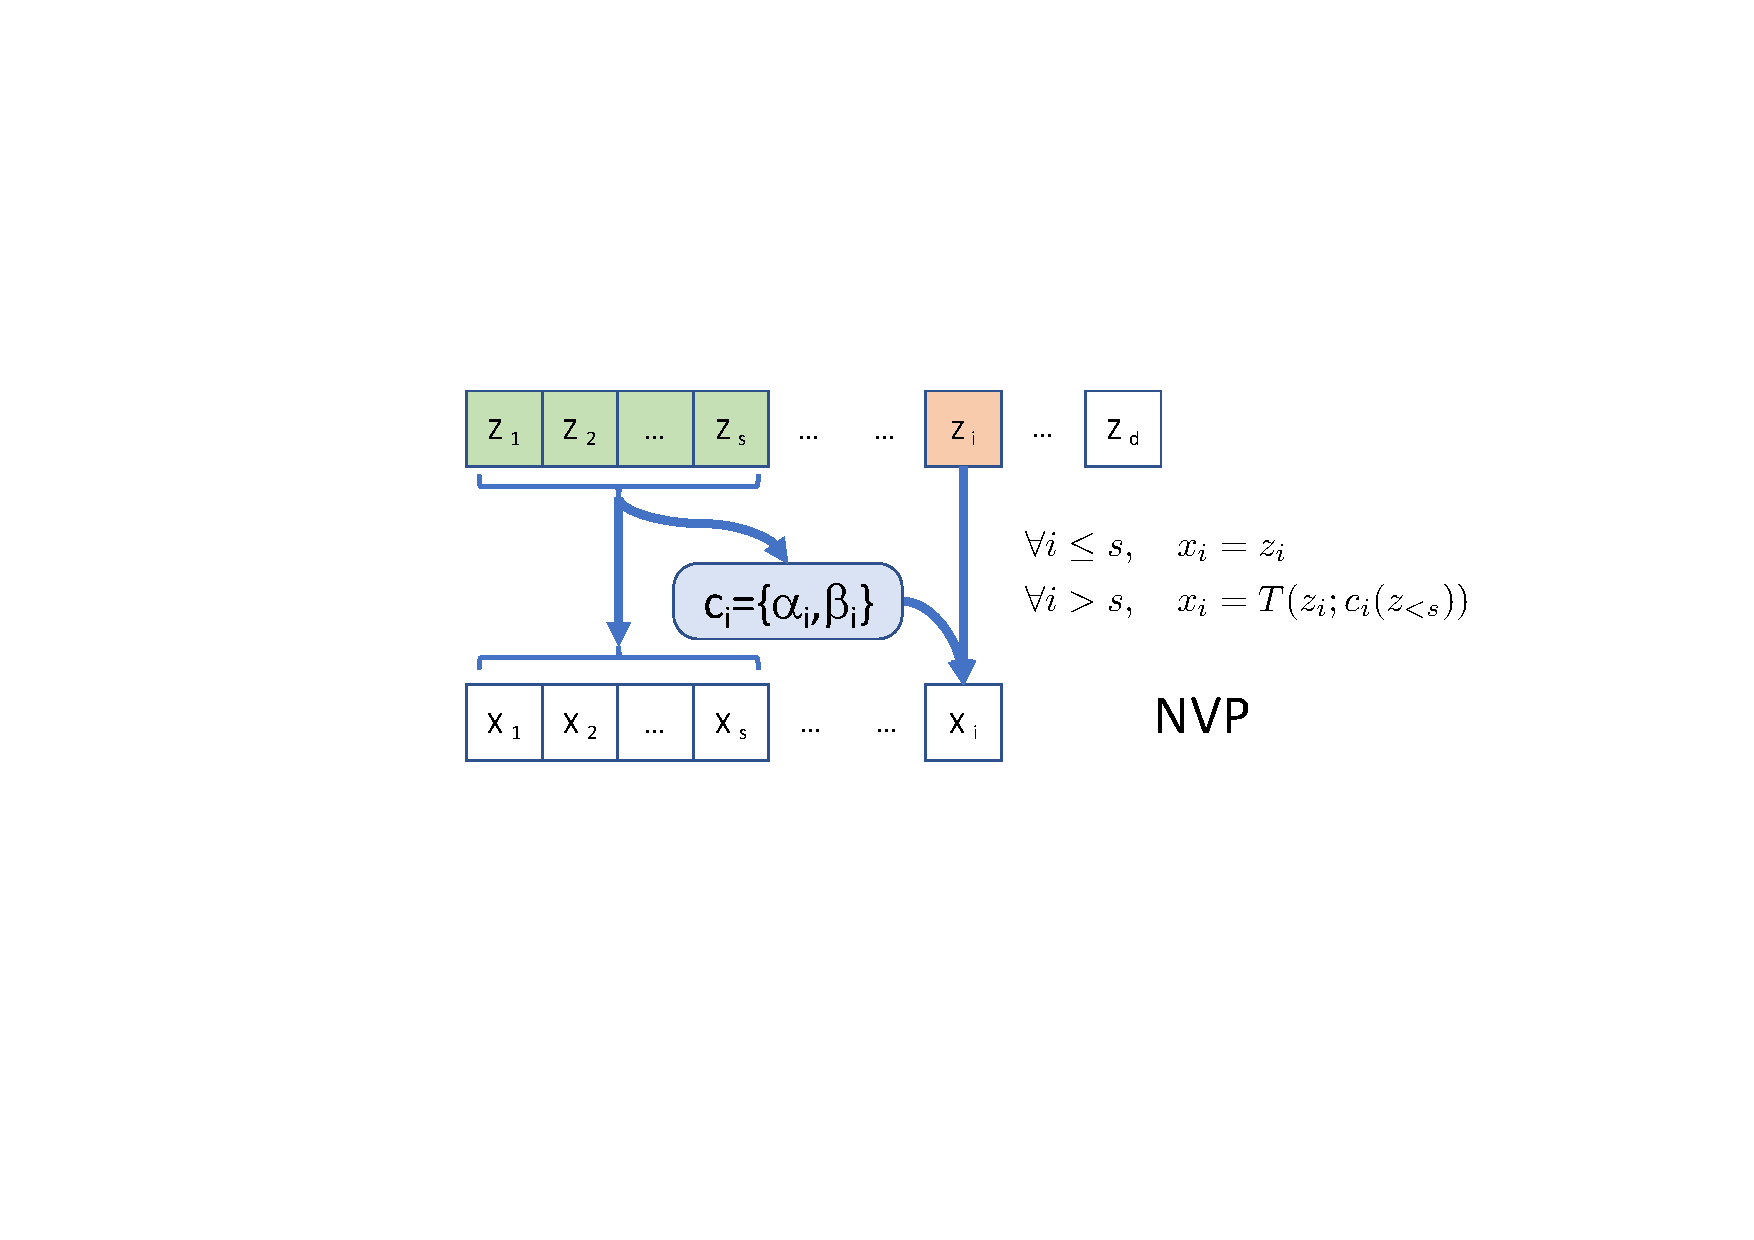
\includegraphics[width=0.45\columnwidth]{fig-nvp.pdf}
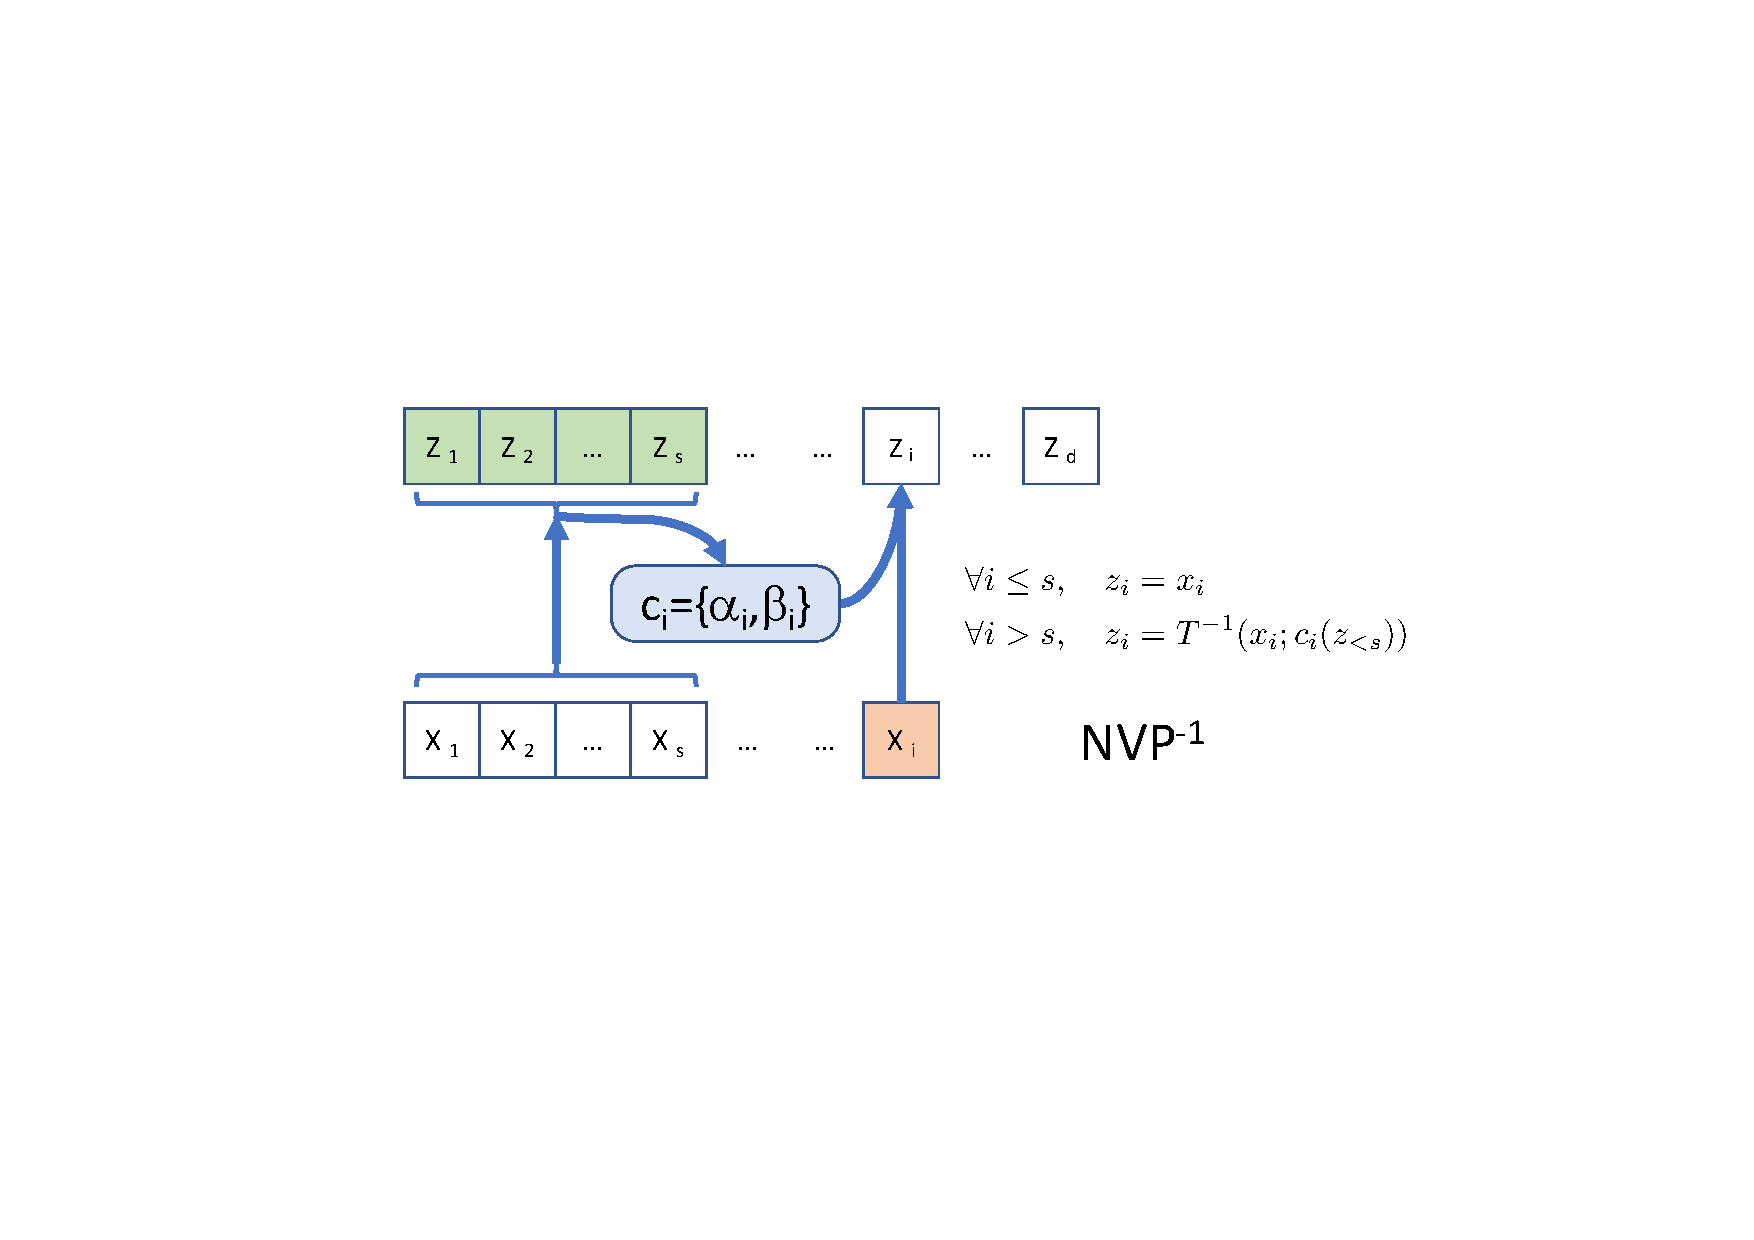
\includegraphics[width=0.45\columnwidth]{fig-nvp-inverse.pdf}
\caption{Affine coupling layer schema of forward and backward directions (Eqs.~\ref{eq-NVP_forward},\ref{eq-NVP_backward}) with a single split mechanism (figure inspired by \cite{Papamakarios2021}).}
\label{fig-nvp}
\end{figure}
%
This splitting schema implemented in a so-called \textit{coupling layer} makes the flow-based model computationally efficient and using deep neural networks, one can achieve complex $(\bm{\alpha},\bm{\beta})$ functions. Now, designers of complete architectures can compose different \textit{coupling layers} by reversing $\bm{z}$ elements between layers to ensure that all elements are transformed at the end of the set of operations. An generalisation of any permutation ordering of the inputs can be performed using a $1\times 1$ convolution layer. \cite{2016arXiv160508803D} improves the modelling using a multi-scale approach which would be prohibitive to describe here, and \cite{Kingma2018} use all these extensions to build the \texttt{Glow} model whose schema is displayed on Figure \ref{fig-Glow-archi}.
\begin{figure}
    \centering
    \vspace{-0cm}
    \begin{subfigure}[b]{0.45\textwidth}
    \begin{center}
        \centering
        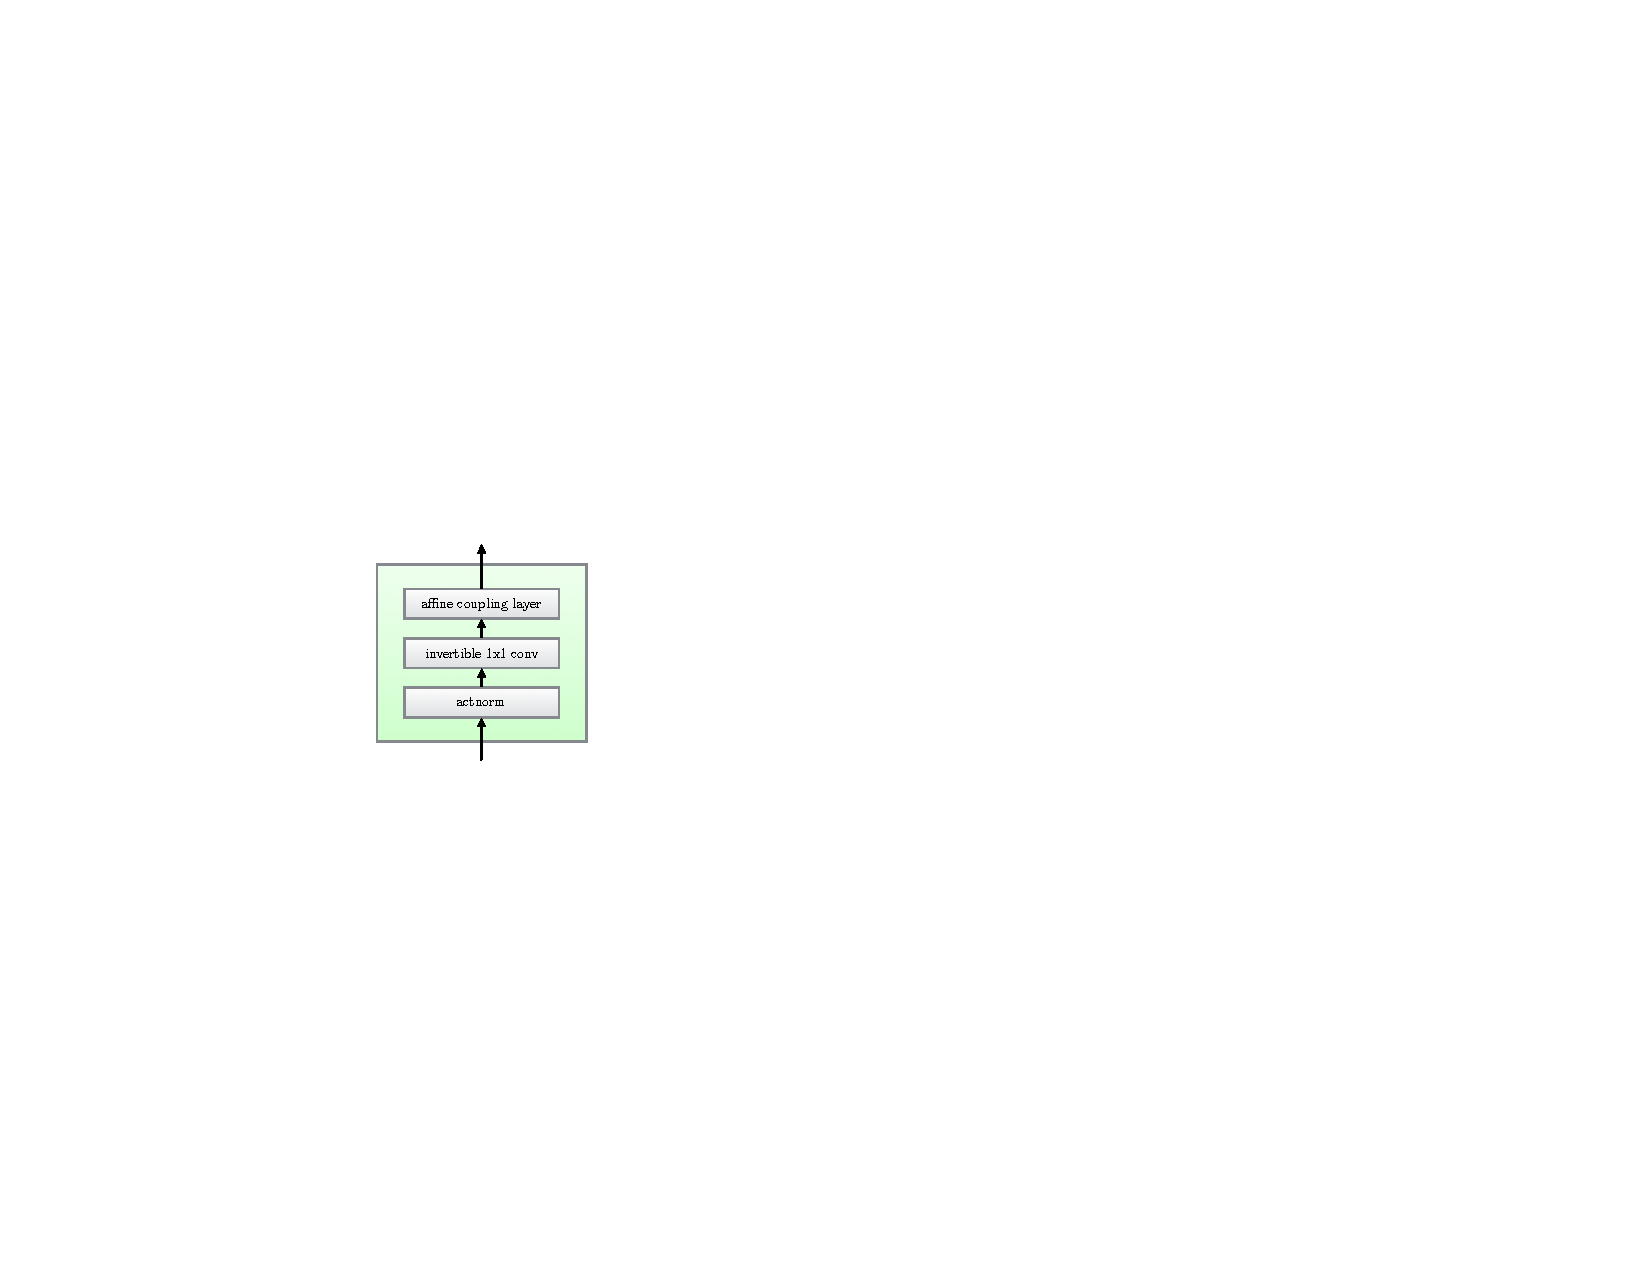
\includegraphics[width=.7\textwidth]{fig-Glow-1.pdf}
        \caption{One step of Glow flow.}
    \end{center}
    \end{subfigure}%
    \vspace{5mm}
    \begin{subfigure}[b]{0.45\textwidth}
        \centering
        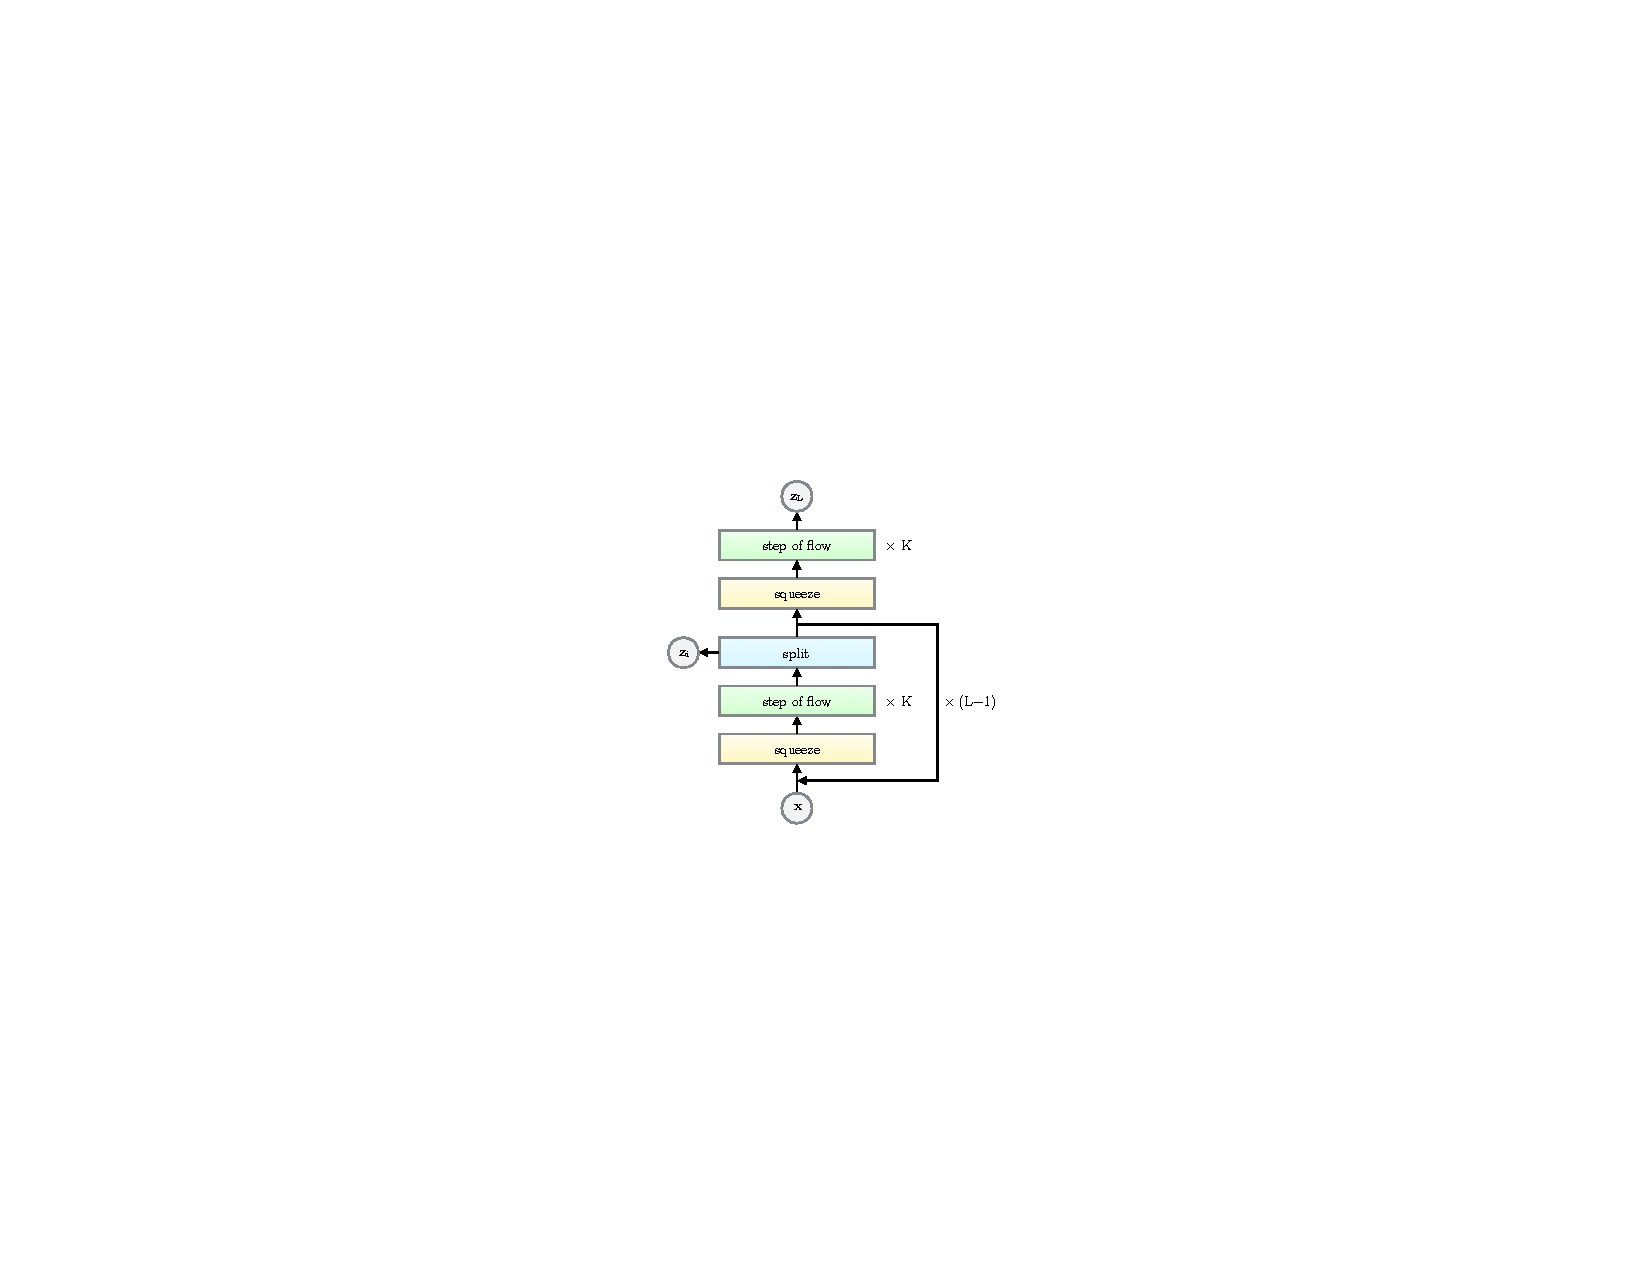
\includegraphics[width=.99\textwidth]{fig-Glow-2.pdf}
        \caption{Multi-scale architecture \citep{2016arXiv160508803D}.}
    \end{subfigure}
    \caption{Figure from \citep{Kingma2018}. The flow step is composed of a scale and bias layer with data dependent initialization (\texttt{actnorm}), a $1\times 1$ invertible convolution layer and an affine coupling layer with $(\bm{\alpha},\bm{\beta})$ issued from a shallow convolutional neural network. Both $\bm{x}$ and $\bm{y}$ are tensors of
shape $[h \times w \times c]$ with spatial dimensions $(h, w)$ and channel dimension $c$ ans $(i, j)$ denote
spatial indices into tensors $\bm{x}$ and $\bm{y}$.  This flow step is embedded in a multi-scale  architecture which has $K$ flow steps and a number of levels $L$ \citep{2016arXiv160508803D}. The squeezing operation reduces a $s \times s \times c$ tensor  into a $s/2\times s/2 \times 4c$ tensor which mix spatial and channel components. At each scale, each channel image is divided into $2\times 2$ patches ($s=2$) and each patch is squeezed. }
    \label{fig-Glow-archi}
\end{figure}
 %
\subsection{Score based diffusion models}
%
To generate samples from $p(\bm{x})$, we can proceed as follows \citep[e.g][]{Chang2023,LinYang2023}. Starting from a sample $\bm{x}_0$ assumed to be drawn from the distribution $p_0(\bm{x})=p(\bm{x})$, we progressively transform it until the  distribution is as simple as for instance $\mathcal{N}(\bm{z},\bm{0},\bm{1})$.  The idea is then to reverse the process (the \textit{backward} mode) by generating a new sample from a new instance of noise. This transfer mapping looks very similar in concept as normalizing flows. Their latent spaces have the same dimension as the data space, but the main difference consists in the fact that the later are deterministic by essence while the former are stochastic. 

Following the notations used in \cite{kadkhodaie2024generalization}, the transport process used in the \textit{score diffusion} algorithm is the Ornstein-Uhlenbeck equation \citep{Uhlenbeck1930}. The \textit{forward} process follows the following stochastic differential equation:
\begin{equation}
d\bm{x}_t = -\bm{x}_t dt + \sqrt{2}\ dB_t \quad t\in[0,T]
\label{eq-Ornstein-cont}
\end{equation}
where $dB_t$ is a Wiener process (Brownian motion) and $T$ is a finite ending time that would be considered to be large enough. The solution of such forward process reads
\begin{equation}
\bm{x}_t = \bm{x}_0 e^{-t} + \underbrace{(1-e^{-2t})^{1/2}}_{\sigma_t} \bm{z} \qquad \bm{z} \overset{iid}{\sim} \mathcal{N}(\bm{z},\bm{0},\bm{1})
\end{equation}
The associated probability density function is given by the expression 
\begin{equation}
p_t(\bm{x}_t) = \int p_t(\bm{x}_t,\bm{x}_0) d\bm{x}_0 = \int p_t(\bm{x}_t|\bm{x}_0) p_0(\bm{x}_0)dx_0
\label{eq-smoothing-p0-gauss}
\end{equation}
where according to the Fokker-Planck representation of the Ornstein-Uhlenbeck process,  it yields
\begin{equation}
p_t(\bm{x}_t|\bm{x}_0)= \frac{1}{(2\pi \sigma_t^2)^{d/2}}\exp\left\{\displaystyle -\frac{\|\bm{x}_t-\bm{x}_0e^{-t}\|^2}{2\sigma_t^2}\right\}
\end{equation}
So, $p_t(\bm{x}_t)$ is the result of the convolution of the initial distribution $p_0(x_0)$ with a Gaussian with variance $\sigma_t^2$ which gradually tends towards the normal distribution $\mathcal{N}(.,\bm{0},\bm{1})$, producing a progressive blurring that also makes $p_t(\bm{x}_t)$ converging towards the normal distribution. 


Notice that in a VAE architecture beyond the information compression,  the transformation from $\bm{x}_0$ to $\bm{z}$ is performed by an \textit{encoder} whose implementation is typically a deep neural networks with trained parameters. This is not the case in the above stochastic process where only noise is added to the original signal (e.g. galaxy image). In the same spirit, the VAE \textit{decoder} or the inverted flows are replaces by stochastic differential equation (damped Langevin)
\begin{equation}
dx_{T-t} = (x_{T-t} + 2\nabla_x \log p_{T-t}(x_{T-t}))dt + \sqrt{2}\ dB_t \quad t\in[0,T]
\label{eq-backward-diffusion}
\end{equation}
where $\nabla_x \log p_{t}(\bm{x}_{t})$ is the \textit{score} of the probability density at time $t$. This backward process is the $\bm{x}=\bm{x}_0$ generative direction from $\mathcal{N}(\bm{z},\bm{0},\bm{1})$ sampling. 

The key problem is how to obtain the score. One can think about two possible approaches: either we have a model for $p_t$ \citep[e.g.][]{Guth2022b,Lempereur2024} that can exploit regularity patterns and assumptions about correlations to provide a constrained parametric framework for learning the score by score matching \citep{hyvarinen2005a}, or we use a \textit{denoising} neural network as introduced by \cite{Bengio2013} and then \cite{Sohl-Dickstein2015,Ho2020} and recently studied from a mathematical point of view by \citep{kadkhodaie2024generalization}, as well as used in cosmology such as the generation of galaxy images \citep{smith2021}, the generation of 21cm luminosity temperature maps \citep{Zhao2023} and super-resolved large-scale cosmic structure predictions \citep{Schanz2023} and sampling of the high-dimensional Bayesian posterior of the weak lensing mass-mapping problem \citep{Remy2023}.

Denoising diffusion stochastic models have certain advantages compared to GAN architecture.


They can jointly be interplayed as for instance in \citep{zhang2021diffusion,gong2021interpreting}.  


%
\section{Experiment}



\section{Discussion}


\section*{Acknowledgements}

\section*{Codes}

%%%%%%%%%%
\addcontentsline{toc}{section}{References}
% Put your bibiliography file here
%\section{Bibliography}
\bibliographystyle{aa}%{elsarticle-harv}%%{mnras}
\bibliography{refs.bib}
%%%%%%%%%%%%%%%%%%%%%%%%%%%%%%%%%
\appendix
\section{Details on the dataset}


\end{document}
